\chapter{Biometrics}
\label{chap:Biometrics}

This chapter presents the concepts related to Biometrics and the security issues related. Section \ref{sec:IntroBiome} presents what is a biometric authentication system. Section \ref{sec:AttacksBiometric} presents the main threats in a biometric authentication system. Finally, Section\ref{sec:FinalRemarks} presents the Final Remarks of the chapter.

\section{Introduction to Biometric Systems}
\label{sec:IntroBiome}

Biometrics is the science of recognizing the identity of a person based on their physical attributes and / or behavior, such as face, fingerprints, hand veins, voice or iris \cite{li2011handbook}. The use of biometrics as authentication factor has some advantages. Naturally, is not possible to forget or transfer a biometric trait and it hardly disappears (perhaps in case of a seriously accidents). Biometrics has some drawbacks, of course. Compared with regular authentication systems, such as passwords or tokens, which are precise, biometric authentication systems have probabilistic behavior. It turns out that there is no perfect match in biometrics; the authentication systems have to deal with error rates. These errors rates can vary by a number of factors. As an example, our voice vary drastically  when we get sick or when we are under stress and this impacts a speaker authentication system. Aging, illumination, pose and face expressions are classical problems in face authentication systems, and these factors impacts the error rates of a face authentication systems. 

The aforementioned problems and other issues are widely studied by the research community \cite{flynn2008handbook}. To use a biometric trait in a biometric system, the candidate must satisfy the following requirements.

\begin{itemize}
        \item Universality (every person must have it);
        \item Uniqueness (must distinguish people);
        \item Stability (must be stable along the time);
        \item Collectability (must be measure);
        \item Performance (must be relatively precise);
        \item Acceptance (the user must acept);
        \item Circumvention (low risk of frauds).
\end{itemize}

Table \ref{tb:comparacao} shows a comparative between the most used biometric traits \cite{maltoni2009handbook}. It can be observed that none of the presented biometric traits fulfill all the listed requirements and the selection of a trait depends of some factors such as, the security requirements and the application purpose \cite{jain1999biometrics}.

\begin{table}[ht]
\caption[Comparison of the most used biometric traits]{Comparison of the most used biometric traits \cite{maltoni2009handbook}}
\begin{center}
    \begin{tabular}{ | c | c | c | c | c | c | c | c |}
    \hline
    \textbf{Biometric trait} & \rotatebox{90}{\textbf{Universality}} & \rotatebox{90}{\textbf{Uniqueness}} & \rotatebox{90}{\textbf{Stability}} & \rotatebox{90}{\textbf{Coletability}} & \rotatebox{90}{\textbf{Performance}} & \rotatebox{90}{\textbf{Acceptance}} & \rotatebox{90}{\textbf{Circunvention}} \\ \hline
    Face                             & High      & Low  & Medium & High     & Low  & High      & Low \\ \hline
    Fingerprint                  & Medium  &  High    & High      & Medium & High     & Medium  & Medium \\ \hline
    Hand geometry         & Medium  & Medium & Medium & High     & Medium & Medium  & Medium \\ \hline
    Palm vein                   & Medium  & Medium  & Medium & Medium & Medium & Medium & High \\ \hline
    Iris                               & High      & High       & High     & Medium & High     & Low  & High \\ \hline
    Signature                   & Low   & Low   & Low  & High     & Low  & High     & Low \\ \hline
    Voice                           & Medium  & Low   & Low  & Medium & Low  & High     & Low \\ \hline
    \end{tabular}
\end{center}
\label{tb:comparacao}
\end{table}

\section{Attacks in Biometric Systems}
\label{sec:AttacksBiometric}

A regular biometric authentication system can be represented with the simple flow chart in Figure \ref{fig:diagram_attacks}.
\begin{figure}[!htb]
\begin{center}
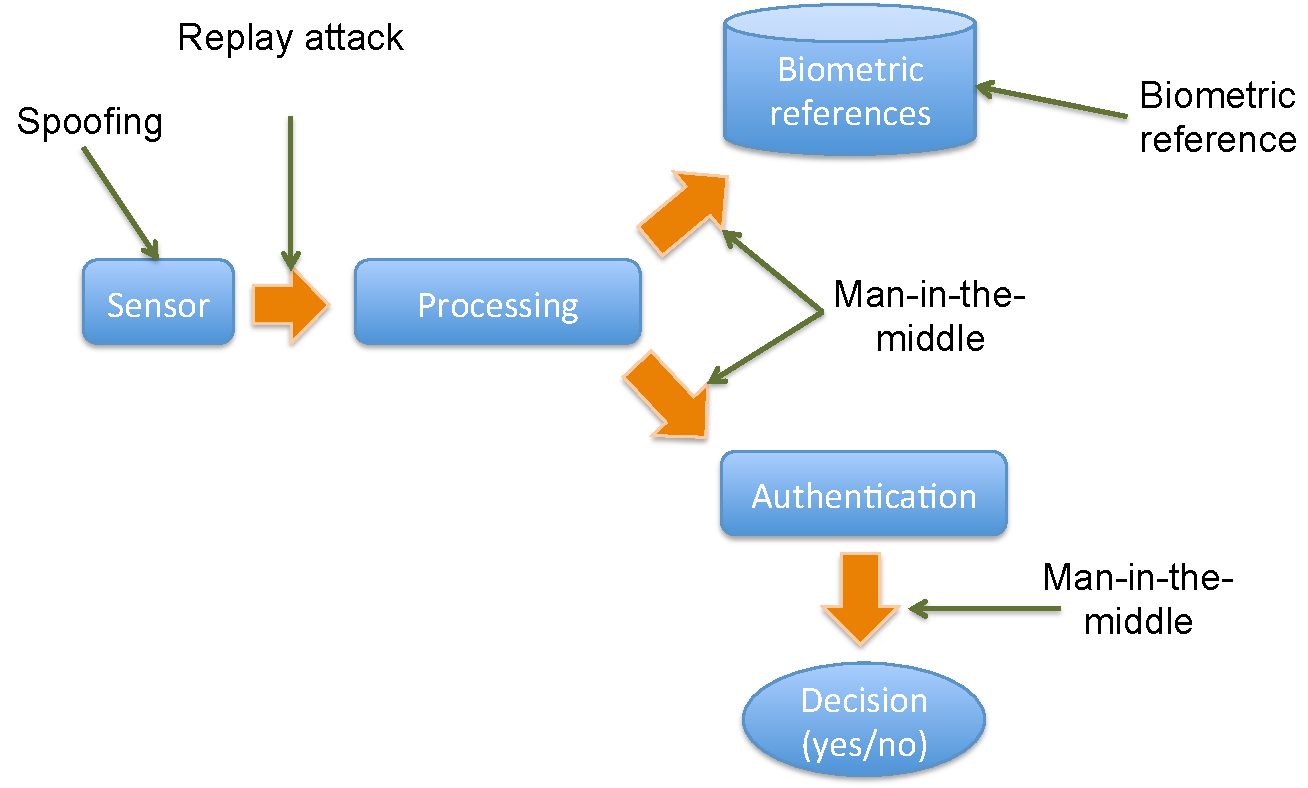
\includegraphics [width=14cm] {images/diagram_attacks.pdf}
\caption[]{Simple architecture of a regular biometric authentication system (adapted from \cite{xiao2005security})} \label{fig:diagram_attacks}
\end{center}
\end{figure}

Firstly the biometric trait is captured using some sensor. Secondly the captured biometric trait is processed in order to extract the biometric features. When it is in an enrollment procedure, these features will generate a biometric reference, and it will be stored in a database. In an authentication procedure, these features will be used in a comparison with the stored biometric reference. It is possible to observe, in the same Figure, that attacks can be done in any point of the architecture \cite{xiao2005security}. The next subsections discusses about each one of the possible point of attacks and how to mitigate it.


\subsection{Replay attack}
\label{sec:rep}

The replay attack is performed by injecting a biometric data previously sent, of the target identity, in order to have a non authorized access. This data can be obtained sniffing the biometric authentication software. To mitigate this kind of attack, the biometric system should ensure that the provided data was not injected artificially \cite{xiao2005security}. The most  popular way of protect this kind of attack is to associate a timestamp to the data. As it is improbable to have the exactly the same biometric data in different times, this method is quite effective.

\subsection{Biometric reference attack}

The attack in the biometric reference is performed where the biometrics are stored. This kind of attack include actions such as the inclusion, removing, modifying and steal biometric references. Among this actions, the possibility to steal a biometric reference is the most dangerous treat, since it is possible to work in a reverse engineering process to regenerate the biometric trait. 

Using a hill climbing technique to optimize to the position and the orientation of the minutia \cite{MartinezDiaz2006} and \cite{hill2001risk} shown that is possible to generate synthetic fingerprints compatible with fingerprints stored in a database. Fake fingers (with a real fingerprint) with gummy or silicon can be generated with this minutia. It is possible also to inject these minutia in the \textbf{Processing} module (Figure \ref{fig:diagram_attacks}) in order to deceive the authentication system. 

To mitigate the risk of this kind of attack best practices in security recommends to encrypt the biometric references and to increase the policy to access these biometric references. 

\subsection{Man-in-the-middle}

In the man in the middle attack, the biometric data is intercepted in any point of the architecture in Figure \ref{fig:diagram_attacks}.  As shown in the Figure \ref{fig:diagram_attacks}, the attacker can:
\begin{itemize}
        \item Manipulate the matching score;
        \item Manipulate the biometric authentication response;
        \item Steal biometric data;
        \item Inject face biometric data (as shown in the Section \ref{sec:rep}).
\end{itemize}

The same security recommendations aforementioned to deal with this security breaks can be used here i.e. encrypt the data before transmission increase the security grants and so on. 

\subsection{Ataque de Spoofing}

The spoofing attack in biometric system is a direct attack to the biometric sensor i.e. a forged biometric trait is presented to the biometric sensor. The goal is to pretend to be someone else in order to get some forbidden privileges. This type of attack is described with more details in Chapter \ref{chap:Spoofing}.

Several technologies related to information security can be deployed in a biometric authentication system in order to mitigate the attacks aforementioned. We can highlight:
\begin{itemize}
        \item Encrypt the biometric data;
        \item Traffic the biometric data using a secure channel;
        \item Deploy all modules of the architecture in a device that cannot be broken;
        \item Using more than one authentication factor.
\end{itemize}
However, in a spoofing attack, the target is the biometric sensor, and in the architecture presented in Figure \ref{fig:diagram_attacks}, is not possible to apply any of the security tools to prevent this king of attack, becoming the most fragile point. This kind of attack is the main point of this thesis.

\section{Final Remarks}
\label{sec:FinalRemarks}

This chapter described the main concepts and the main threats that a biometric authentication system can suffer. As aforementioned, the biometric sensor is the most fragile point of threats in the architecture presented in the Figure \ref{fig:diagram_attacks}. Countermeasures need to be studied in order to mitigate these threats. This masters thesis will deal with that topic.

